

\tikzset{every picture/.style={line width=0.75pt}} %set default line width to 0.75pt        

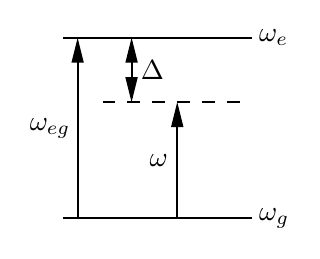
\begin{tikzpicture}[x=0.75pt,y=0.75pt,yscale=-1,xscale=1]
%uncomment if require: \path (0,300); %set diagram left start at 0, and has height of 300

%Straight Lines [id:da18819191009761904] 
\draw    (81,129) -- (172,129) ;
%Straight Lines [id:da1376948784583416] 
\draw    (81,216) -- (172,216) ;
%Straight Lines [id:da21818736070050204] 
\draw    (136,162) -- (136,216) ;
\draw [shift={(136,160)}, rotate = 90] [fill={rgb, 255:red, 0; green, 0; blue, 0 }  ][line width=0.08]  [draw opacity=0] (12,-3) -- (0,0) -- (12,3) -- cycle    ;
%Straight Lines [id:da6990718420713145] 
\draw  [dash pattern={on 4.5pt off 4.5pt}]  (100,160) -- (172,160) ;
%Straight Lines [id:da6995865544982842] 
\draw    (114,131) -- (114,158) ;
\draw [shift={(114,160)}, rotate = 270] [fill={rgb, 255:red, 0; green, 0; blue, 0 }  ][line width=0.08]  [draw opacity=0] (12,-3) -- (0,0) -- (12,3) -- cycle    ;
\draw [shift={(114,129)}, rotate = 90] [fill={rgb, 255:red, 0; green, 0; blue, 0 }  ][line width=0.08]  [draw opacity=0] (12,-3) -- (0,0) -- (12,3) -- cycle    ;
%Straight Lines [id:da8678920245446373] 
\draw    (88,131) -- (88,216) ;
\draw [shift={(88,129)}, rotate = 90] [fill={rgb, 255:red, 0; green, 0; blue, 0 }  ][line width=0.08]  [draw opacity=0] (12,-3) -- (0,0) -- (12,3) -- cycle    ;

% Text Node
\draw (174,216) node [anchor=west] [inner sep=0.75pt]    {$\omega _{g}$};
% Text Node
\draw (174,129) node [anchor=west] [inner sep=0.75pt]    {$\omega _{e}$};
% Text Node
\draw (117,144.5) node [anchor=west] [inner sep=0.75pt]    {$\Delta $};
% Text Node
\draw (133,188) node [anchor=east] [inner sep=0.75pt]    {$\omega $};
% Text Node
\draw (86,172.5) node [anchor=east] [inner sep=0.75pt]    {$\omega_{eg} $};


\end{tikzpicture}
